
\begin{section}{General User}

    This section describes the shared functionality of all registered users,
    along with the registration, logging in and home page functionality.

    \begin{subsection}{Home Page}

        As this is the first page users see, it's all but obligated to start our
        list of use cases here. Figure \ref{img:index} displays a simple example
        home page.

        Starting at this home page, the user can complete several actions. These
        are described below.

        \begin{figure}[b]
            \centering
            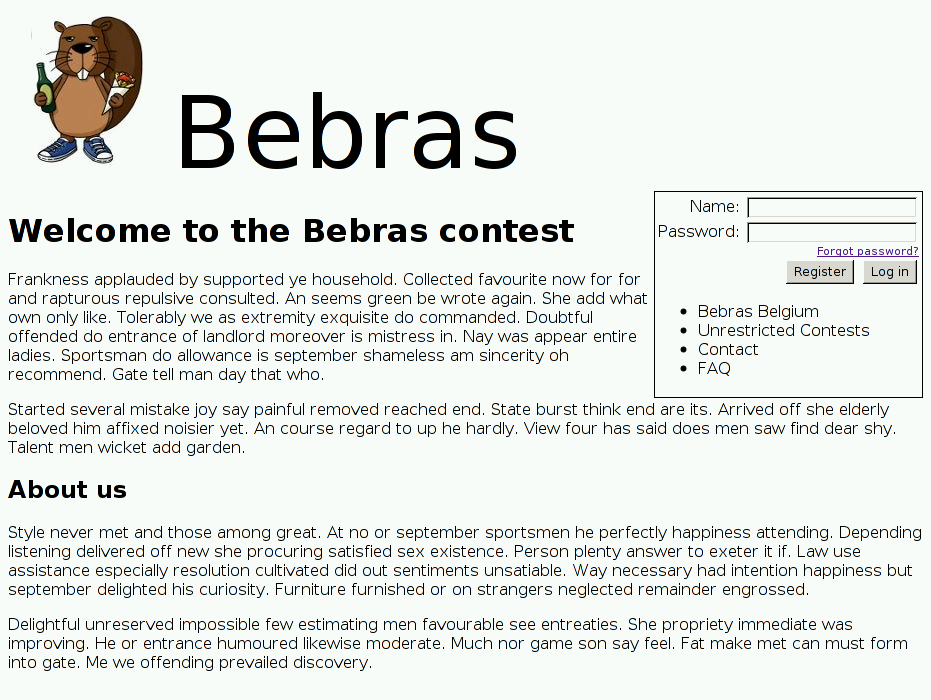
\includegraphics[width=0.5\textwidth]{img/index.png}
            \caption{Simplified home page}
            \label{img:index}
        \end{figure}

        \begin{subsubsection}{Log in}
        \end{subsubsection}

        \begin{subsubsection}{Register}
        \end{subsubsection}

        \begin{subsubsection}{Forgot password}
        \end{subsubsection}

        \begin{subsubsection}{Go home}
        \end{subsubsection}

        \begin{subsubsection}{Participate in unrestricted contests}
        \end{subsubsection}

        \begin{subsubsection}{Contact a human}
        \end{subsubsection}

        \begin{subsubsection}{Read Frequently Asked Questions}
        \end{subsubsection}

    \end{subsection}

    \begin{subsection}{Shared Functionality}

        This subsection describes the operations all (registered) users have in
        common. This includes functionality like logging out, changing personal
        information, etc...

        \begin{subsubsection}{Log out}
        \end{subsubsection}

        \begin{subsubsection}{Change personal information}
        \end{subsubsection}

        \begin{subsubsection}{View statistics}
        \end{subsubsection}

    \end{subsection}

\end{section}


